% \documentclass{WHUBachelor}% 选项 forprint: 交付打印时添加, 避免彩色链接字迹打印偏淡. 即使用下一行:
\documentclass[forprint]{myreport}
\usepackage{tcolorbox}
\usepackage{listings}
\lstdefinestyle{lfonts}{
    basicstyle = \footnotesize\ttfamily,
    stringstyle = \color{purple},
    keywordstyle = \color{blue!60!black}\bfseries,
    commentstyle = \color{olive}\scshape,
}
\lstdefinestyle{lnumbers}{
    numbers = left,
    numberstyle = \tiny,
    numbersep = 1em,
    firstnumber = 1,
    stepnumber = 1,
}
\lstdefinestyle{llayout}{
    breaklines = true,
    tabsize = 2,
    columns = flexible,
}
\lstdefinestyle{lgeometry}{
    xleftmargin = 20pt,
    xrightmargin = 0pt,
    frame = tb,
    framesep = \fboxsep,
    framexleftmargin = 20pt,
}
\lstdefinestyle{lgeneral}{
    style = lfonts,
    style = lnumbers,
    style = llayout,
    style = lgeometry,
}
\lstdefinestyle{c++}{
	language = {c++},
	style = lgeneral,
}

\begin{document}
%%%%%%%%%%%%%%%%%%%%%%%%%%%%%%%%%%%%%%%%%%%%%%%%%%%%%%%%%%%%%%%%%%%%%%%%%%%%
% 封面
%%%%%%%%%%%%%%%%%%%%%%%%%%%%%%%%%%%%%%%%%%%%%%%%%%%%%%%%%%%%%%%%%%%%%%%%%%%%
\title{homework 3}
\Cschoolname{数据科学与计算机学院}          % 学院名
\Cmajor{计算机科学与技术}                  % 专业中文名
\StudentNumber{16337237} % 填写自己的学号
\author{王永锋}                            % 作者名字
\Csupervisor{陈鹏飞}        %指导教师中文名、职称
\date{二〇一八年五月七日}                % 日期, 要注意和英文日期一致!!
\pdfbookmark[0]{封面}{title}         % 封面页加到 pdf 书签
\maketitle
\frontmatter
%%%%%%%%%%%%%%%%%%%%%%%%%%%%%%%%%%%%%%%%%%%%%%%%%%%%%%%%%%%%%%%%%%%%%%%%%%%%
% 目录
%%%%%%%%%%%%%%%%%%%%%%%%%%%%%%%%%%%%%%%%%%%%%%%%%%%%%%%%%%%%%%%%%%%%%%%%%%%%
% 把目录加入到书签
\pagenumbering{Roman}              % 正文之前的页码用大写罗马字母编号.
\pdfbookmark[0]{目录}{toc}
\tableofcontents
%% 以下是正文
\mainmatter 
%%%%%%%%%%%%%%%%%%%%%%%%%%%%%%%%%%%%%%%%%%%%%%%%%%%%%%%%%%%%%%%%%%%%%%%%%%%%
% 正文
%%%%%%%%%%%%%%%%%%%%%%%%%%%%%%%%%%%%%%%%%%%%%%%%%%%%%%%%%%%%%%%%%%%%%%%%%%%%

\chapter{第一题}

%\newtcolorbox{mybox}{}
%\renewtcolorbox{mybox}{colback = red!25!white, colframe = red!75!black}
%\begin{mybox}[title = {}]
\begin{tcolorbox}[title = {第一题}]
Consider a simple loop that calls a function dummy containing a programmable delay.All invocations of the function are independent of the others. Partition this loop across four threads using static, dynamic, and guided scheduling. scheduling. Use different parameters for static and guided scheduling.Document the result of this experiment as the delay within the dummy function becomes large.
\end{tcolorbox}

\section{题目分析}

这一道题,主要需要我们探讨这样的几个问题。

\begin{itemize}
    \item 对于\texttt{dynamic}调度方法,选取怎样的\texttt{chunk size}能够得到更高的加速比。
    \item 对于\texttt{guided}调度方法,选取怎样的\texttt{chunk size}能够得到更高的加速比
    \item 对不同的调度方法的加速比进行横向的比较。
\end{itemize}

\section{实验前提}

\subsection{延迟函数设计}

本次实验所使用的延迟主要来自于这样的一个双重循环:
%\usepackage{listings}
\begin{lstlisting}[style = c++]
void parallel_delay(int times){
    # pragma omp parallel
    {
        num_threads = omp_get_num_threads();
        # pragma omp for schedule(runtime)
        for (int i = 0; i < times; i++){
            for (int j = 0; j < times; j++){
                sum += i*j;             
        }
    }
}
\end{lstlisting}

其中循环的次数为$ times * times $,该times 的值在后面的图中表示为$delay\_times$。

因此,可用$delay\_times$的值表示延迟的大小。

\subsection{实验环境}

本次实验在一台CPU为\texttt{i3-3110M},系统为ubuntu的笔记本上测试,该笔记本放在宿舍里挂机,没有运行其他的程序。我通过ssh连接到该电脑中跑代码记录时间,因此可保证运行环境的稳定。

该笔记本CPU为物理双核,因此理论上能够达到的加速比最高为2。

\section{dynamic调度方法}

本节探讨不同的\texttt{chunk size}与\texttt{dynamic}调度方法的加速比之间的关系。

在实验前,我先在网上查了相关资料,了解到在dynamic调度方法中,\texttt{chunk size}的意义为每一次分配给线程的循环次数。又了解到dynamic默认的参数为1,在该参数下,使用该调度方法会极其缓慢,因此在后面,我根据该参数的意义,将研究的\texttt{chunk size}范围大致定在100-4000左右。

实验中,我编写了脚本在电脑中跑程序并记录时间,然后使用python画图以直观的展现加速比与chunk size之间的关系。可见\autoref{fig:e1-dy-full}。

%\usepackage{changepage}
%\usepackage{rotating}
%\usepackage{float}
%\usepackage[section]{placeins}
%\begin{sidewaystable}[!Htp]
\begin{figure}[htp]
    %\begin{adjustwidth}{-1.5cm}{-1cm}
    \centering
    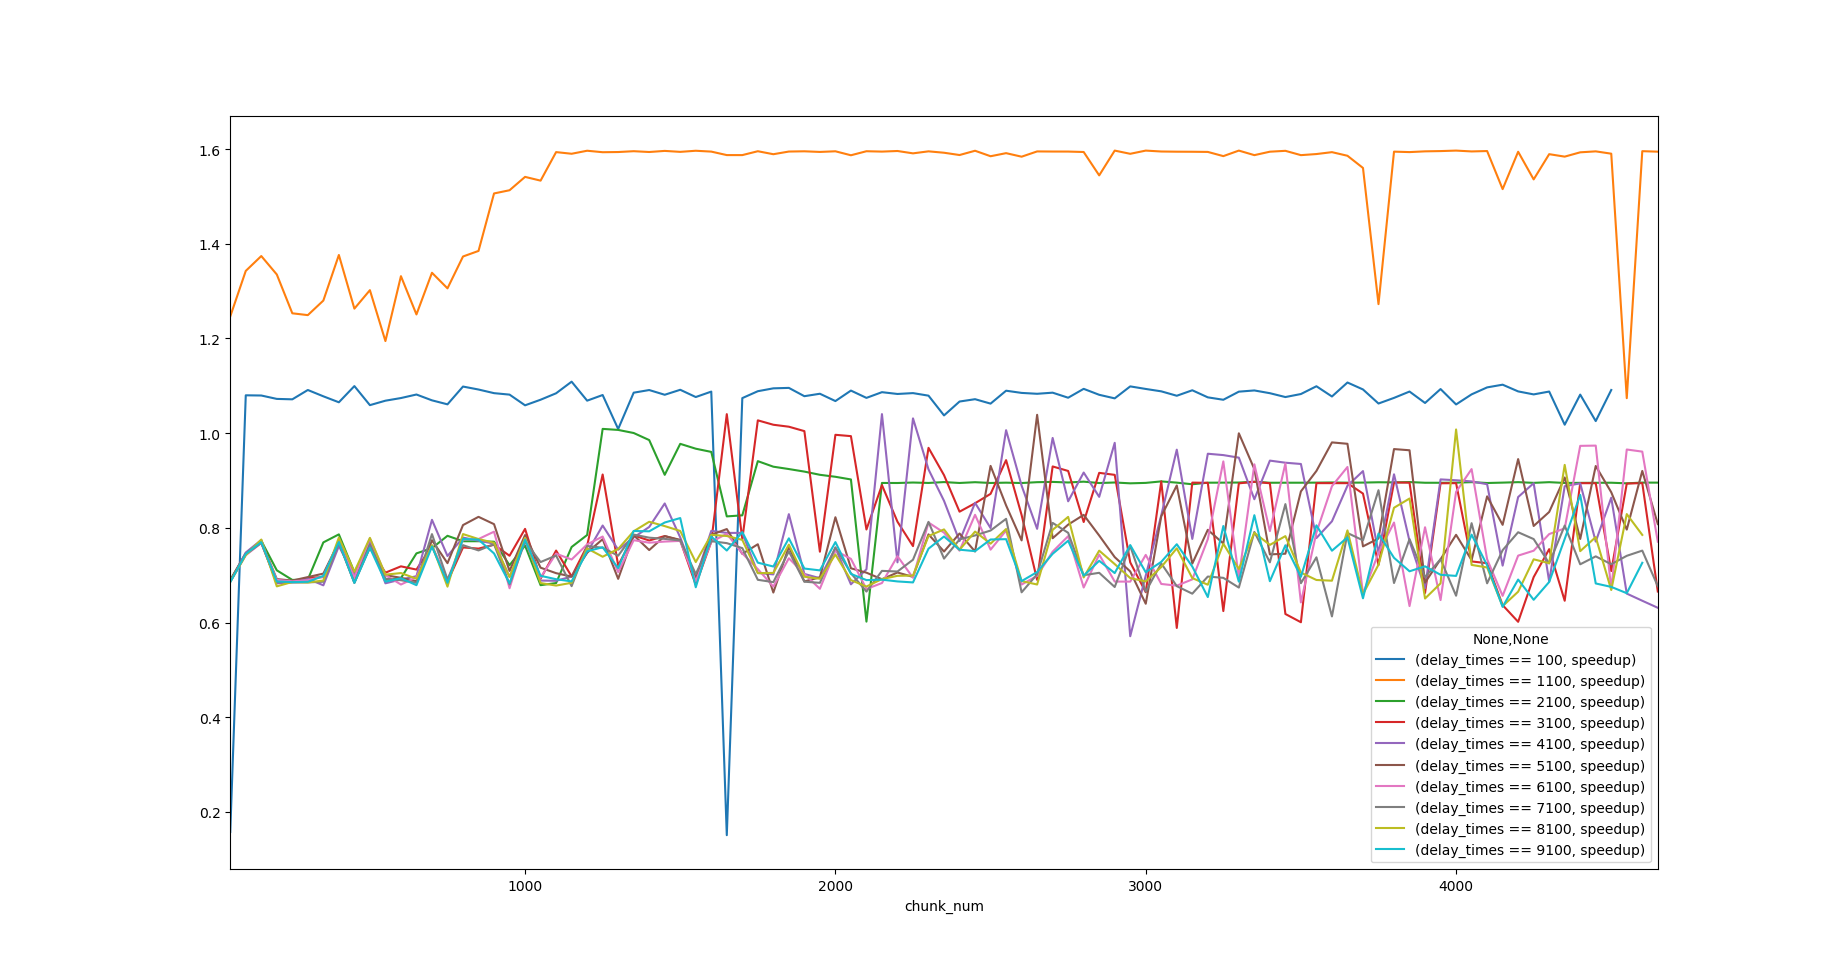
\includegraphics[width=17cm]{"../HW3-1/figure/dynamic_chunk_num.png"}
    \caption{加速比与 chunk size 之间的关系}
    \label{fig:e1-dy-full}
    %\end{adjustwidth}
\end{figure}

为了更精确的展现结果,我将横坐标的范围缩小,得到新的图,可见\autoref{fig:e1-dy-to-2000}。

%\usepackage{changepage}
%\usepackage{rotating}
%\usepackage{float}
%\usepackage[section]{placeins}
%\begin{sidewaystable}[!Htp]
\begin{figure}[htp]
    %\begin{adjustwidth}{-1.5cm}{-1cm}
    \centering
    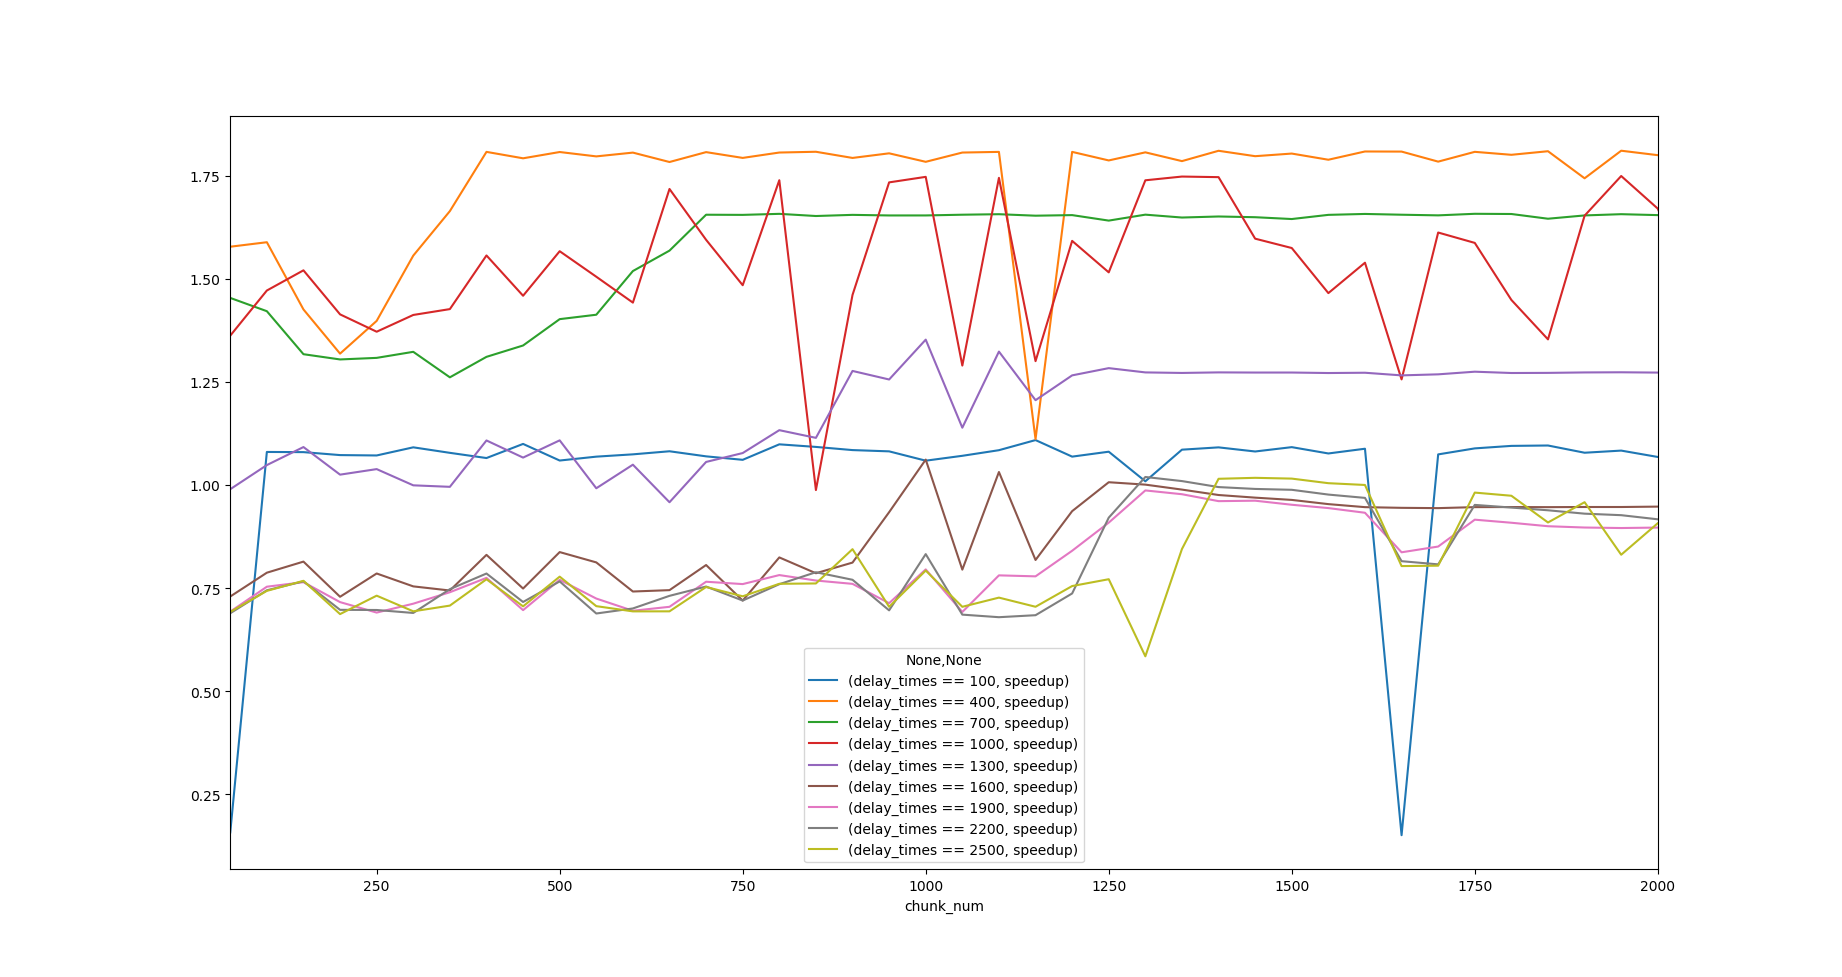
\includegraphics[width=17cm]{"../HW3-1/figure/dynamic_chunk_num100-2000.png"}
    \caption{加速比与chunk size 之间的关系}
    \label{fig:e1-dy-to-2000}
    %\end{adjustwidth}
\end{figure}

\subsection{实验结果}

\begin{itemize}
    \item 在延时比较小的时候,(如\autoref{fig:e1-dy-to-2000}中橙线),使用适当的chunk size 可以显著的提高运行速度。
    \item 通过\autoref{fig:e1-dy-to-2000}中绿线和橙线的比较,可以知道,当延时变大的时候,要使用更大的chunk size才可以达到更好的加速效果。
    \item 当延时越来越大的时候,并行程序的加速效果渐渐弱化,甚至不如串行程序。
\end{itemize}

\section{guided调度方法}

本节研究不同的\texttt{chunk size}对guided调度方法效果的影响。

需要注意到,在\texttt{guided}调度方法中,\texttt{chunk size}参数的意义是最终分配的迭代数收敛到的值。guided调度方法对每次分配的迭代数的处理方式为指数级收敛,收敛速度很快,若很快就收敛到1,而剩余未分配的迭代数仍有许多,这时候便会如先前提到的默认dynamic一样,导致运行时间变长。

因此,我根据参数的意义,选取了一个合适的范围进行研究。结果如\autoref{fig:e1-gu-to-1500}所示。

%\usepackage{changepage}
%\usepackage{rotating}
%\usepackage{float}
%\usepackage[section]{placeins}
%\begin{sidewaystable}[!Htp]
\begin{figure}[htp]
    %\begin{adjustwidth}{-1.5cm}{-1cm}
    \centering
    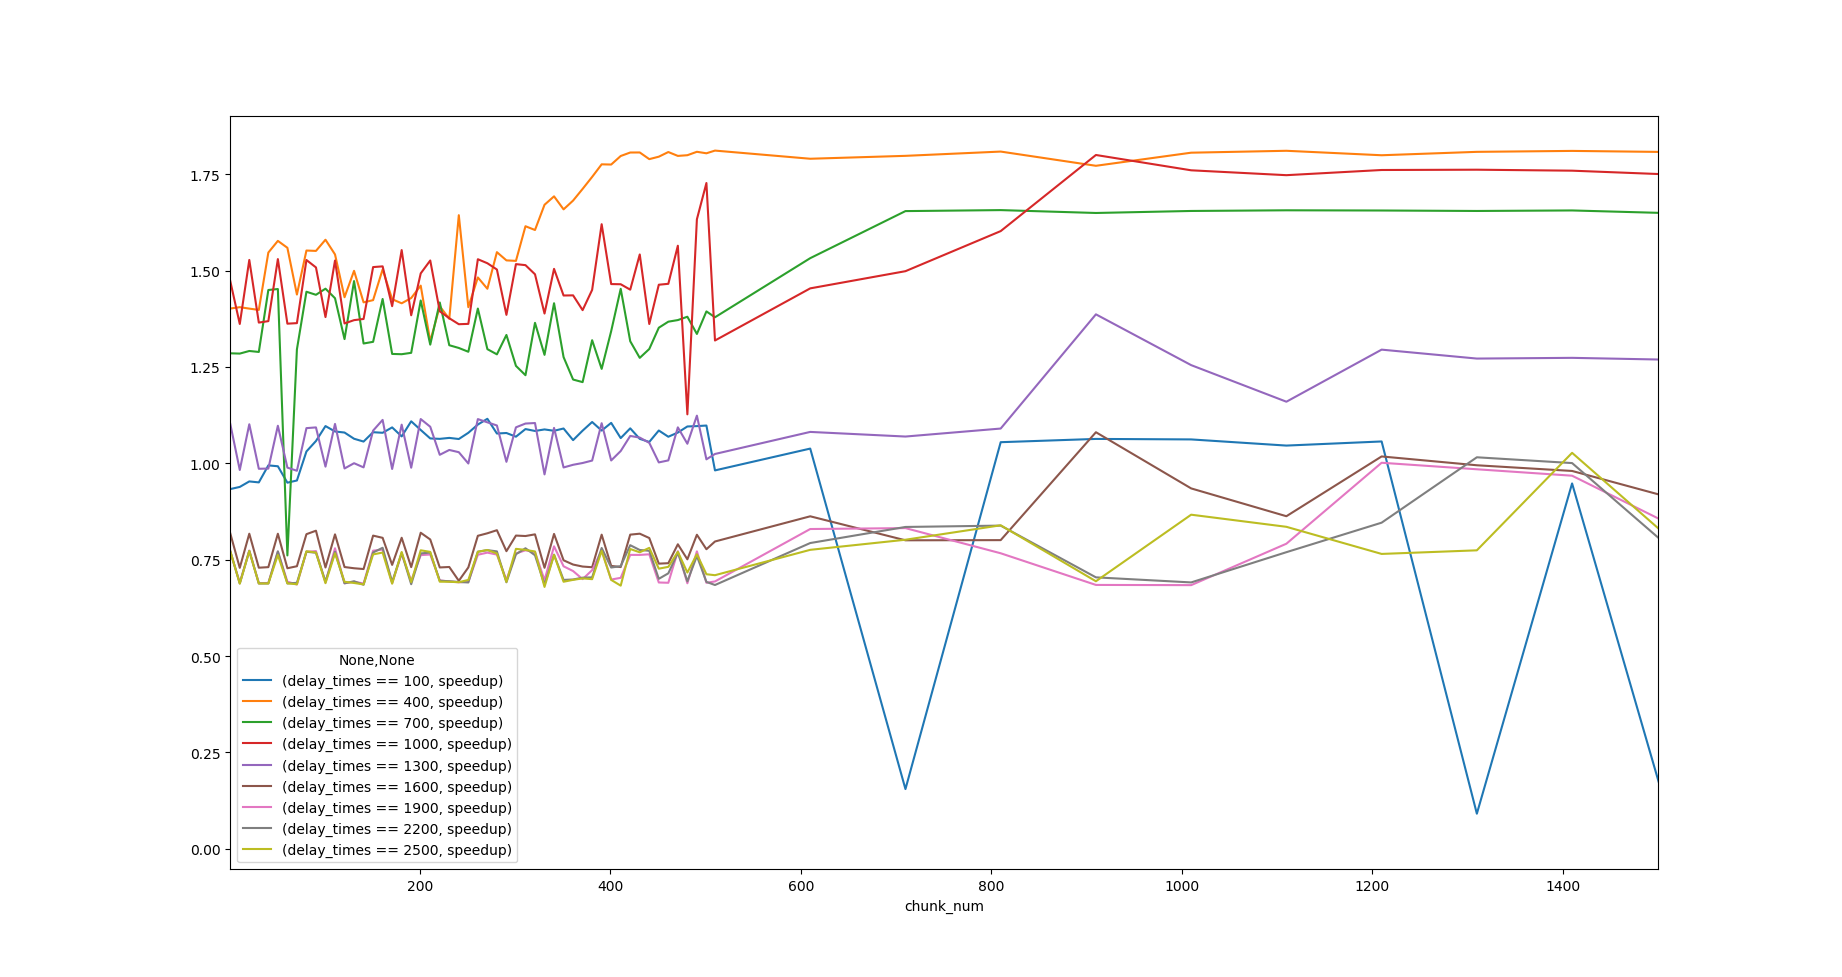
\includegraphics[width=15cm]{"../HW3-1/figure/guided_chunk_num1-1500.png"}
    \caption{guided调度方法中,加速比与chunk size 之间的关系}
    \label{fig:e1-gu-to-1500}
    %\end{adjustwidth}
\end{figure}


\subsection{实验结果}

\begin{itemize}
    \item 在延迟较小的情况下(delay\_times 在100到1000之间),多线程程序的加速效果是比较明显的。
    \item 在一定范围内,随着延迟的增大,需要更大的\texttt{chunk size}才能够达到理想的加速效果。
    \item 当延迟过大时,并行程序的加速效果渐渐消失,甚至不如串行程序。
\end{itemize}

\section{不同调度方法之间的对比}

\texttt{OpenMP}中,主要由这三种调度方法:

\begin{itemize}
    \item \texttt{static}
    \item \texttt{dynamic}
    \item \texttt{guided}
\end{itemize}

其中,我需要说明一下上面没有研究static调度方法的原因。static调度方法在默认情况下是将循环的迭代数平均分配给每一个线程,而我认为这已经做到足够好,在此基础上,无论是分配的迭代数再增加,还是减少,都会带来额外的分配的开销。相比起static,其他两种调度方法对参数的选择就要灵活很多,加速效果也不清晰,因此需要研究。

\subsection{作图}

从上面对两个调度方法的研究来看,我在这一次研究中,对\texttt{dynamic}调度方法,选取的\texttt{chunk size}为1000,而在\texttt{guided}调度方法中则选取910。

下面做出程序加速比随\texttt{delay\_times}增加而变化的趋势图,如\autoref{fig:e1-all-speedup-time-full}。

%\usepackage{changepage}
%\usepackage{rotating}
%\usepackage{float}
%\usepackage[section]{placeins}
%\begin{sidewaystable}[!Htp]
\begin{figure}[htp]
    %\begin{adjustwidth}{-1.5cm}{-1cm}
    \centering
    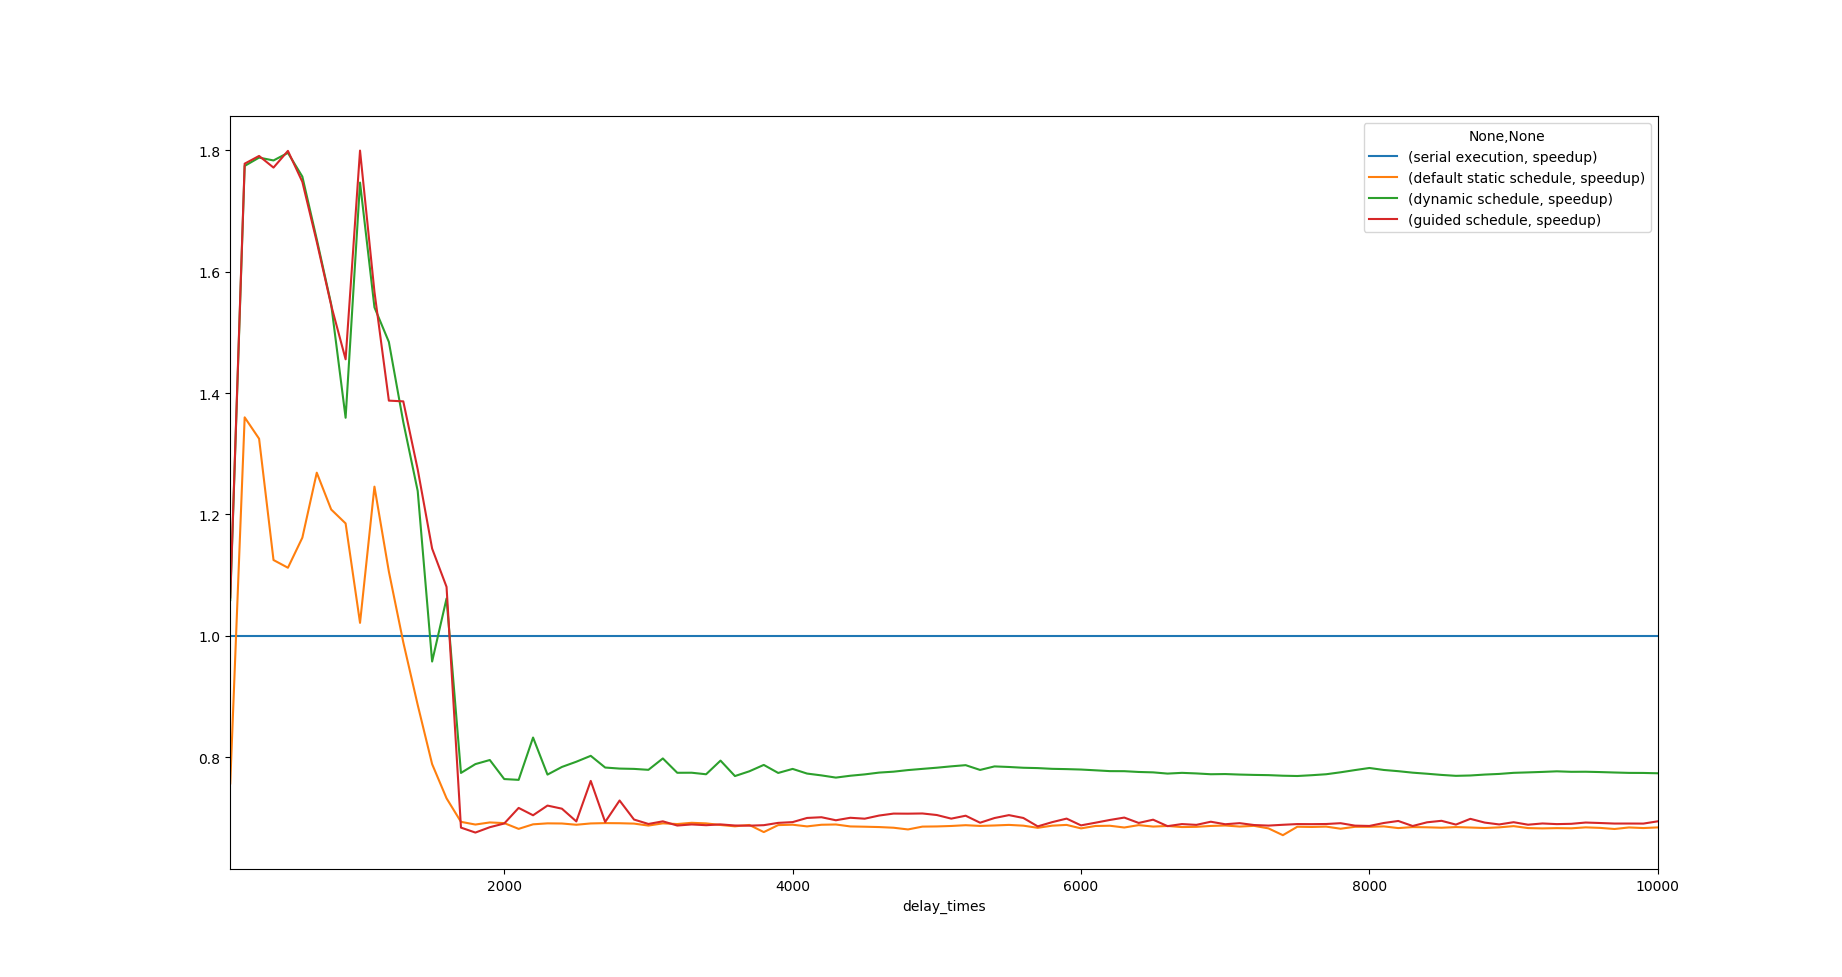
\includegraphics[width=15cm]{"../HW3-1/figure/all_to10000.png"}
    \caption{程序加速比与运行延时之间的关系。}
    \label{fig:e1-all-speedup-time-full}
    %\end{adjustwidth}
\end{figure}

放大前面一段更有意义的数据,如\autoref{fig:e1-all-speedup-time}所示。

%\usepackage{changepage}
%\usepackage{rotating}
%\usepackage{float}
%\usepackage[section]{placeins}
%\begin{sidewaystable}[!Htp]
\begin{figure}[htp]
    %\begin{adjustwidth}{-1.5cm}{-1cm}
    \centering
    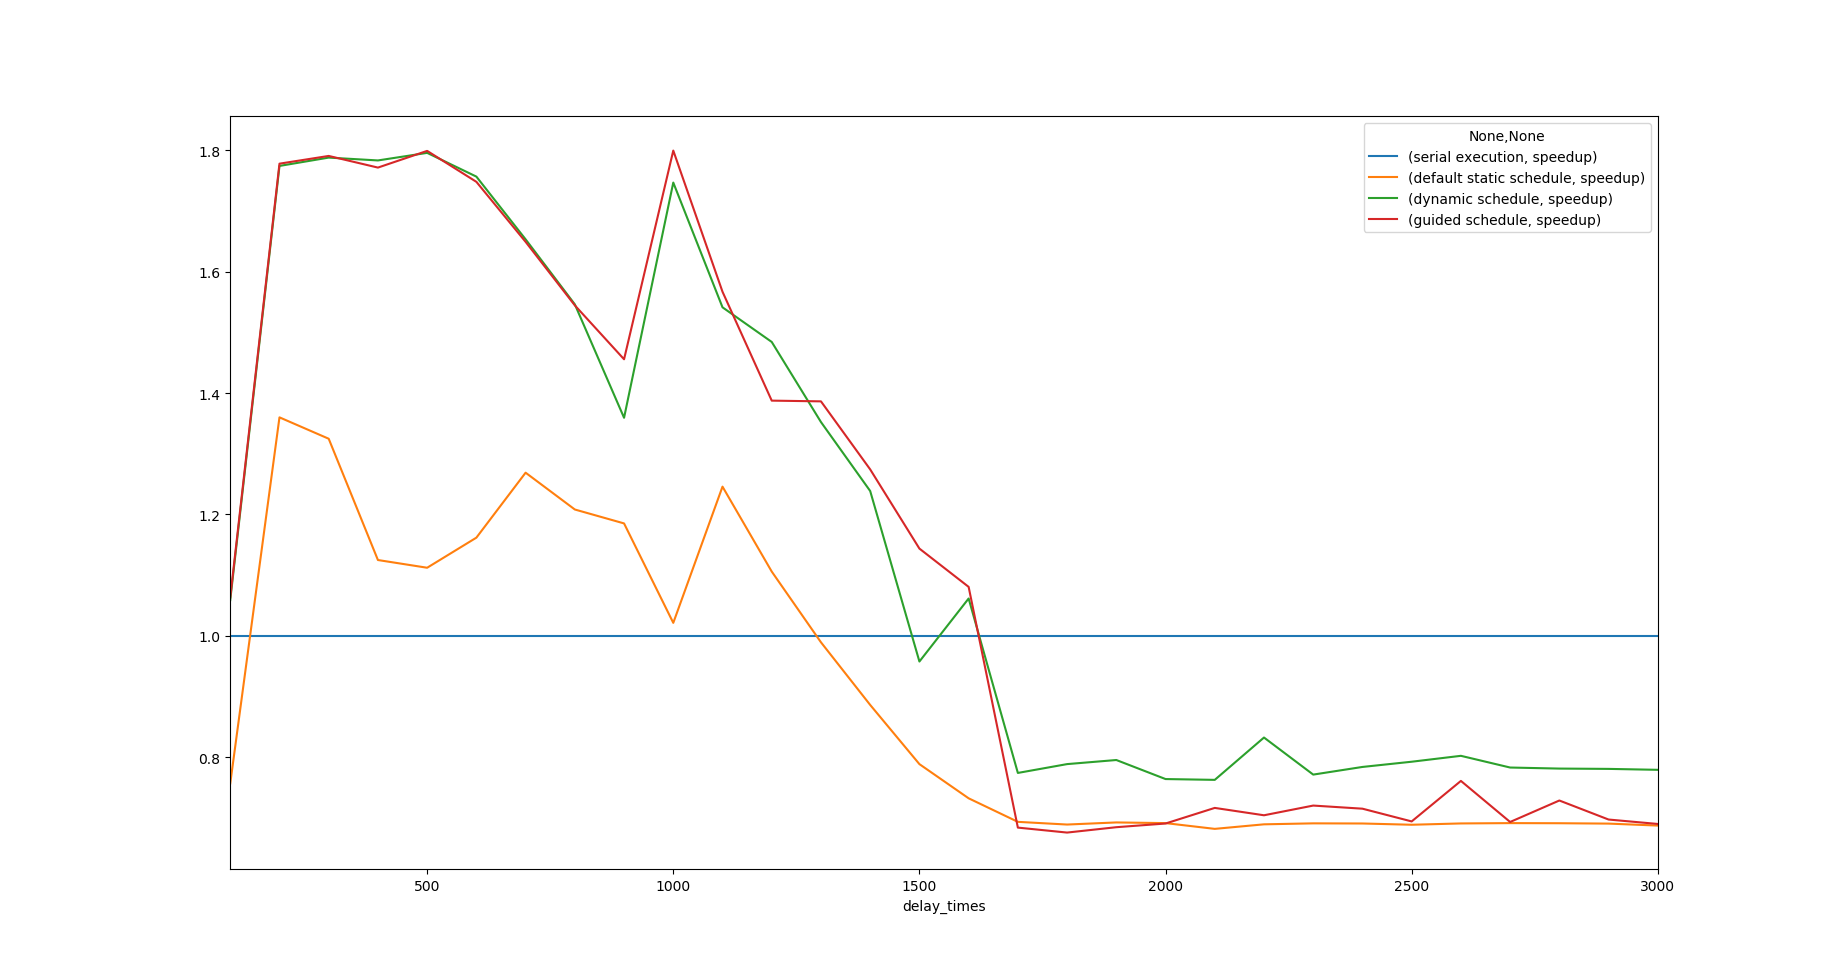
\includegraphics[width=15cm]{"../HW3-1/figure/all_2.png"}
    \caption{程序加速比与运行延时之间的关系。}
    \label{fig:e1-all-speedup-time}
    %\end{adjustwidth}
\end{figure}

\subsection{实验结果}

\begin{itemize}
    \item 在一定范围的延时内,三种调度方法均达到了不错的加速效果,其中dynamic和guided都达到了加速比为1.8的程度,接近极限值2。
    \item static调度方法表现不如dynamic与guided调度方法,dynamiac调度方法与guided调度方法表现类似。
    \item 这些调度方法在延时超过一定大小时,会渐渐失去加速效果,运行时间甚至不如串行程序。
\end{itemize}

\chapter{第二题}

%\usepackage{tcolorbox}
%\newtcolorbox{mybox}{}
%\renewtcolorbox{mybox}{colback = red!25!white, colframe = red!75!black}
%\begin{mybox}[title = {}]
\begin{tcolorbox}[title = {第二题}]
Implement and test the OpenMP program for computing a matrix-matrix (50 * 50) product. Use the OMP\_NUM\_THREADS environment veriable to control the number of threads and plot the performance with varying numbers of threads. Consider three cases in which
\begin{itemize}
    \item only the outermost loop is parallelized.
    \item the outer two loops are parallelized.
    \item all three loops are parallelized.
\end{itemize}
What is the observed result from these three cases?
\end{tcolorbox}

\section{实验前提}


\subsection{矩阵规模}

在测试过程中发现,50*50的矩阵乘法规模太小,导致在输出时间的时候在大多数情况下只会输出0。出于便于研究,易于对比数据的目的,此后研究的矩阵乘法均是1200维下的矩阵乘法。

\subsection{测试环境}

在我自己电脑进行测试的时候,由于我一边用我自己的电脑完成作业,一边跑程序,跑出来的时间波动过大,看不出规律,因此,对于测试环境,要求要尽可能少的活动进程,本次作业的数据,我是在宿舍的一台没有人用的电脑跑的,保证了运行环境没有过多的其他进程的干扰。

\subsection{运行性能的评价}

本次实验在评价矩阵乘法的性能时,由于并没有会改变矩阵乘法串行时间的因素,因此主要以运行时间来进行评价。

\section{矩阵乘法的实现}


可见代码文件中的`t1.cpp`。除去其他的辅助函数,矩阵乘法的核心部分如此实现。

%\usepackage{listings}
\begin{lstlisting}[style = c++]
void product(){
    # pragma omp parallel for collapse(3)
    // 该参数用于设置并行到哪一个级别的循环
    for (int i = 0; i < MATRIX_SIZE; i++){
        for (int j = 0; j < MATRIX_SIZE; j++){
            for (int k = 0; k < MATRIX_SIZE; k++){
                ans[i][j] += lhs[i][k]*rhs[k][j];
            }
        }
    }
}
\end{lstlisting}


在OpenMP编译指令中,可以见到`collapse`,其后的数字表明并行化的循环层数,根据这个层数,我分为三种情况来研究,这三种情况分别对应题目的三小问。

\begin{itemize}
    \item 情况一:最外层循环并行化
    \item 情况二:两层循环并行化
    \item 情况三:三层循环并行化
\end{itemize}

\subsection{对cache优化的简单矩阵乘法}

考虑到计时不准的缘故,尽量的减少I/O时间能够提高实验结果的准确度。因此我对该矩阵乘法做了一些不影响并行度的对cache友好的优化,再重复进行了一次实验。

优化后的代码如此实现,通过将第二层循环和第三层循环交换位置,提高该矩阵乘法的空间局部性,从而减少程序cache不命中的情况。

%\usepackage{listings}
\begin{lstlisting}[style = c++]
void product(){
    # pragma omp parallel for collapse(3)
    // 该参数用于设置并行到哪一个级别的循环
    for (int i = 0; i < MATRIX_SIZE; i++){
        for (int k = 0; k < MATRIX_SIZE; k++){
            for (int j = 0; j < MATRIX_SIZE; j++){
                ans[i][j] += lhs[i][k]*rhs[k][j];
            }
        }
    }
}   
\end{lstlisting}

\section{实验过程}

当运行线程数控制在1-850范围中时,运行时间随线程数量变化的图如\autoref{fig:e2-time-full}所示。

%\usepackage{changepage}
%\usepackage{rotating}
%\usepackage{float}
%\usepackage[section]{placeins}
%\begin{sidewaystable}[!Htp]
\begin{figure}[htp]
    %\begin{adjustwidth}{-1.5cm}{-1cm}
    \centering
    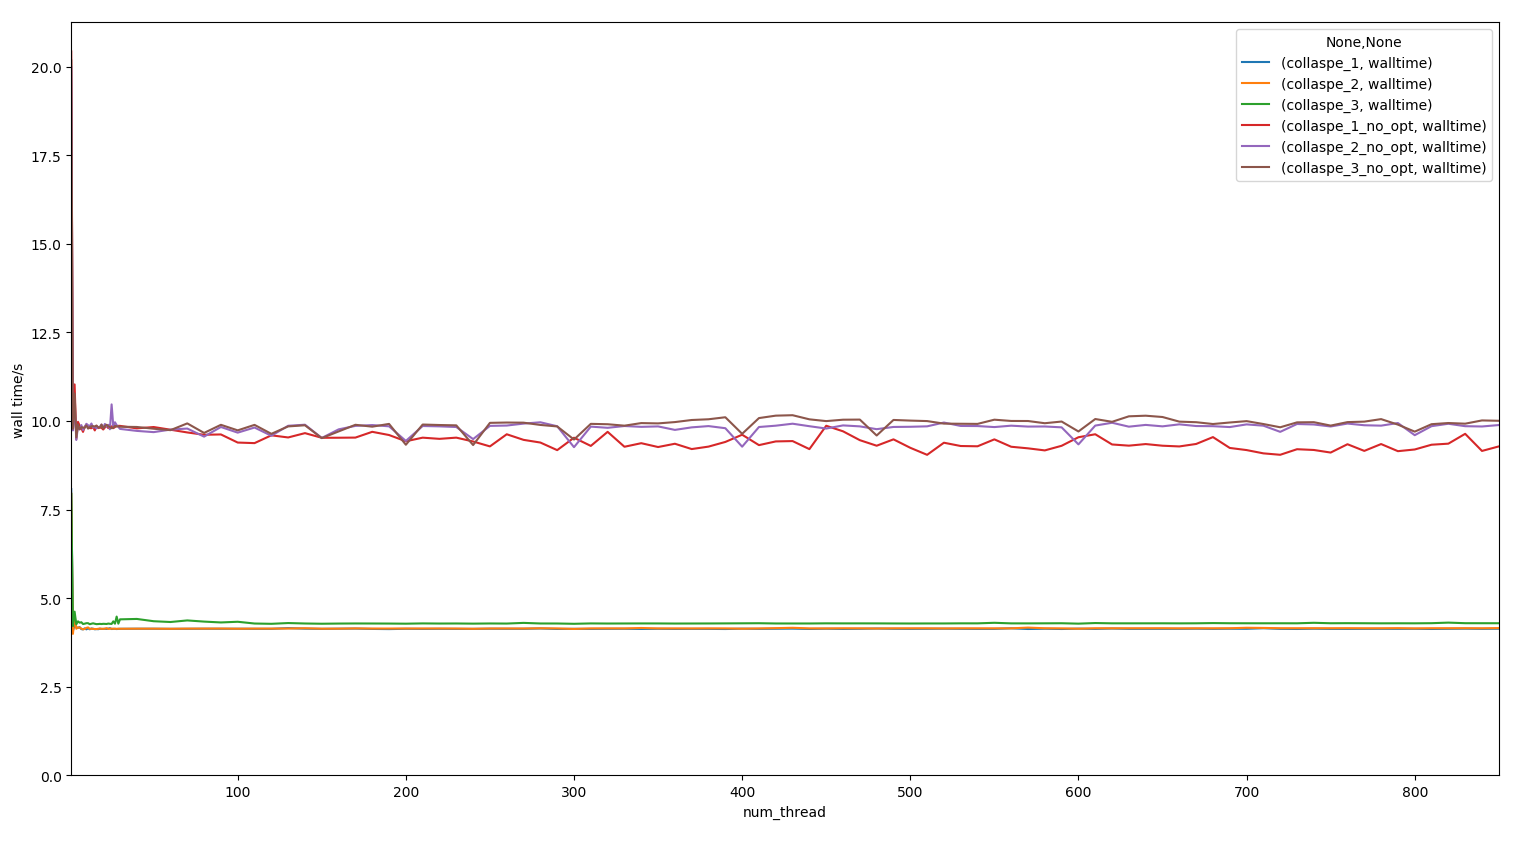
\includegraphics[width=15cm]{"../figure/2018-05-06-16-51-58.png"}
    \caption{运行时间与线程数量之间的关系}
    \label{fig:e2-time-full}
%\end{adjustwidth}
\end{figure}


为了更清晰的展现实验结果,当运行线程数控制在1-30范围中时,运行时间随线程数量变化的图如\autoref{fig:e2-time}所示。
%\usepackage{changepage}
%\usepackage{rotating}
%\usepackage{float}
%\usepackage[section]{placeins}
%\begin{sidewaystable}[!Htp]
\begin{figure}[htp]
    %\begin{adjustwidth}{-1.5cm}{-1cm}
    \centering
    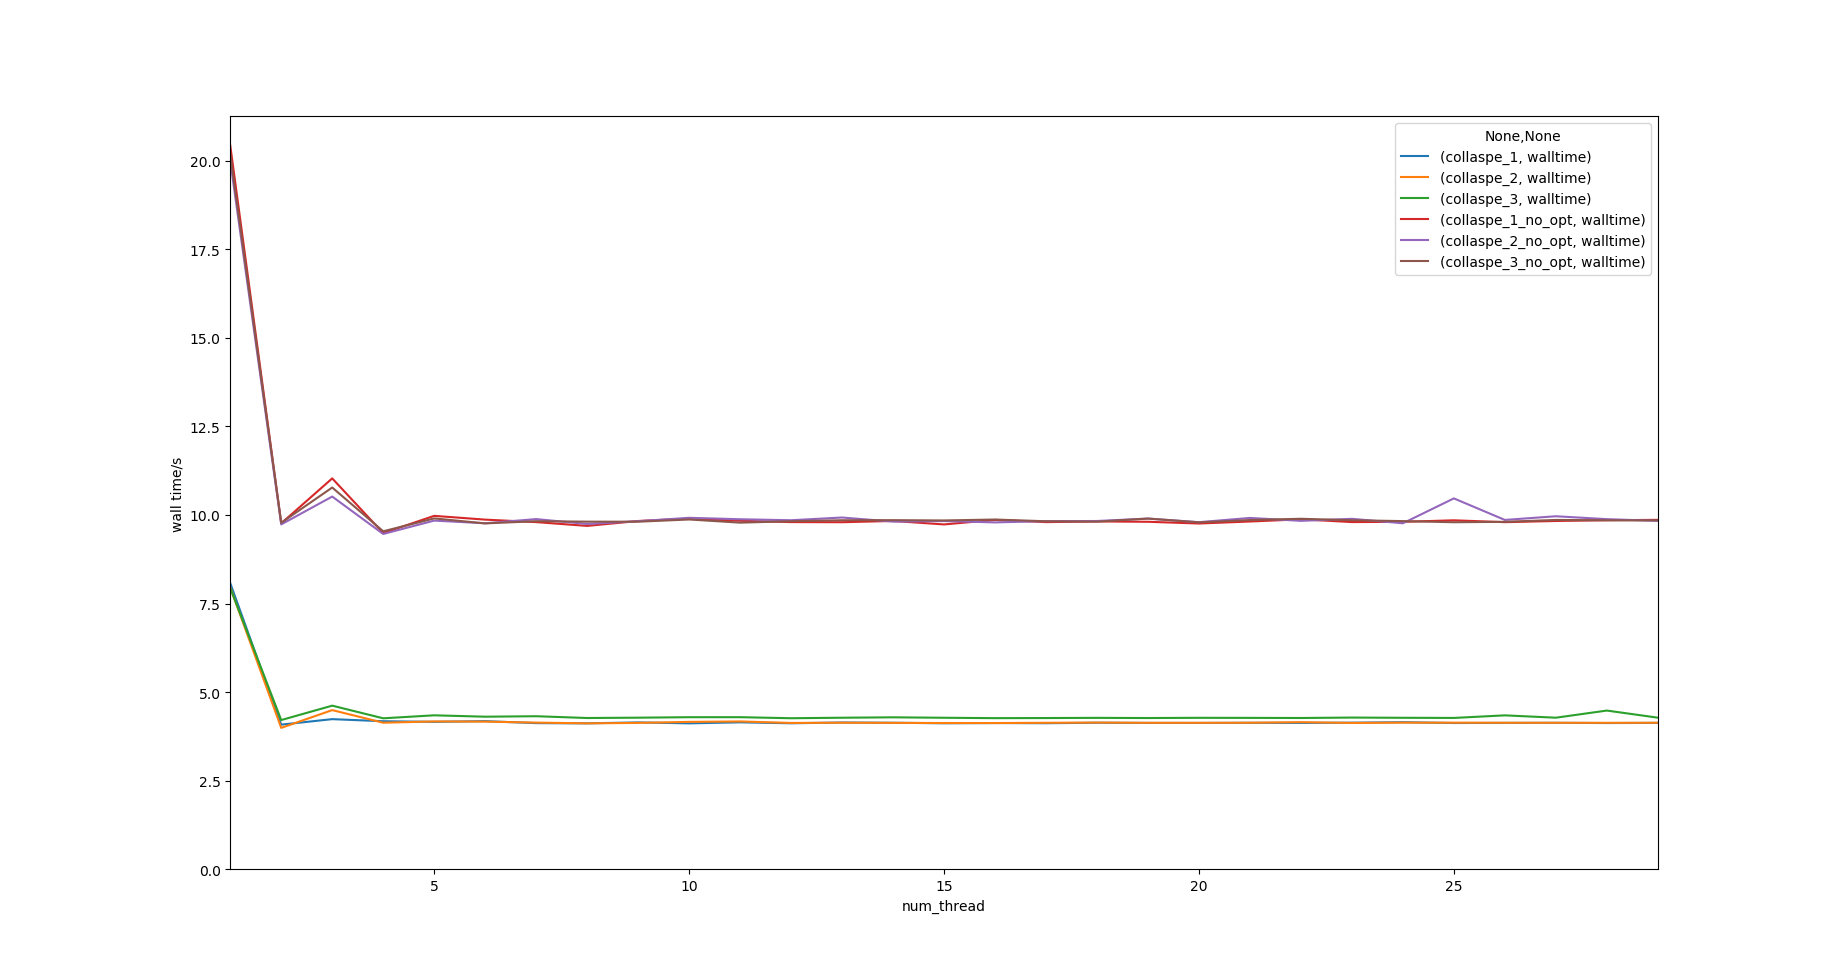
\includegraphics[width=15cm]{"../figure/2018-05-06-16-50-54.png"}
    \caption{运行时间与线程数量的关系}
    \label{fig:e2-time}
    %\end{adjustwidth}
\end{figure}


\section{实验结果}

\begin{itemize}
    \item 在对cache没有优化的矩阵乘法中,运行时间波动大,从中反映的运行时间规律不明确。相对而言,对cache优化后的矩阵乘法总体运行时间波动较小,反映的规律较为可信。
    \item 从对cache优化过的矩阵乘法得出的结果可知,三层循环都并行化时,运行时间总是会比其他两种情况长约3.5%。
    
\end{itemize}



%%%%%%%%%%%%%%%%%%%%%%%%%%%%%%%%%%%%%%%%%%%%%%%%%%%%%%%%%%%%%%%%%%%%%%%%%%%%
% 参考文献
%%%%%%%%%%%%%%%%%%%%%%%%%%%%%%%%%%%%%%%%%%%%%%%%%%%%%%%%%%%%%%%%%%%%%%%%%%%%
% \cleardoublepage\phantomsection
% \addcontentsline{toc}{chapter}{参考文献}

% \bibliography{opsystem}
% \bibliographystyle{unsrt}

% \begin{thebibliography}{00}
%   \bibitem{r1} 作者. 文章题目 [J].  期刊名, 出版年份,卷号(期数): 起止页码.
%   \bibitem{r2} 作者. 书名 [M]. 版次. 出版地:出版单位,出版年份:起止页码.
%   \bibitem{r3} 邓建松等, 《\LaTeXe~科技排版指南》, 科学出版社.
%   \bibitem{r4} 吴凌云, 《CTeX~FAQ (常见问题集)》, \textit{Version~0.4}, June 21, 2004.
%   \bibitem{r5} Herbert Vo\ss, Mathmode, \url{http://www.tex.ac.uk/ctan/info/math/voss/mathmode/Mathmode.pdf}.
% \end{thebibliography}
%%%%%%%%%%%%%%%%%%%%%%%%%%%%%%%%%%%%%%%%%%%%%%%%%%%%%%%%%%%%%%%%%%%%%%%%%%%%
% 附录
%%%%%%%%%%%%%%%%%%%%%%%%%%%%%%%%%%%%%%%%%%%%%%%%%%%%%%%%%%%%%%%%%%%%%%%%%%%%
\appendix

\chapter{文件的组织}

%\usepackage{listings}
\begin{lstlisting}[style = c++]
    .
    ├── figure
    │   ├── 2018-05-06-16-50-54.png
    │   ├── 2018-05-06-16-51-58.png
    │   ├── collapse_1-3_1200_all_to-850.eps
    │   ├── collapse_1-3_1200_no_opt.eps
    │   ├── collapse_1-3_1200_no_opt_to-850.eps
    │   ├── collapse_1-3_1200_opt.eps
    │   └── collapse_1-3_1200_opt_to-850.eps
    ├── HW3-1
    │   ├── a.exe
    │   ├── all_time.csv
    │   ├── a.out
    │   ├── b.exe
    │   ├── figure
    │   │   ├── all_2.png
    │   │   ├── all.png
    │   │   ├── all_to10000.png
    │   │   ├── dynamic_chunk_num100-2000.png
    │   │   ├── dynamic_chunk_num.png
    │   │   ├── gueded_chunk_num1-500.png
    │   │   ├── guided_chunk_num1-1500.png
    │   │   └── guided.png
    │   ├── loop-parallel-schedule.cpp
    │   ├── read_data.py
    │   ├── readme.md
    │   ├── run.sh
    │   └── save.cpp
    ├── HW3-2
    │   ├── all_time.csv
    │   ├── matrix_product.cpp
    │   ├── read_data.py
    │   ├── readme.md
    │   ├── run_all.sh
    │   └── run.sh
    └── report.pdf
\end{lstlisting}


\cleardoublepage
\end{document}